\begin{frame}{Vì sao cần testing và ATPG?}
\begin{itemize}
\item Verification: thiết kế có đúng đặc tả? Testing: chip chế tạo có lỗi?
\item Stuck-at: một dây bị kẹt 0 (SA0) hoặc 1 (SA1).
\item ATPG tìm mẫu làm đáp ứng mạch tốt khác mạch lỗi tại ngõ ra.
\end{itemize}
\begin{block}{Hai điều kiện bắt buộc}
Kích hoạt lỗi tại vị trí lỗi và lan truyền khác biệt đến ngõ ra quan sát được.
\end{block}
\end{frame}

% Sơ đồ c17 dùng cho slide 3 (chỉ số hiệu dây) và slide 4 (có giá trị, đường lỗi đỏ).
\newif\ifPOneVal
\newcommand{\POneLab}[2]{\ifPOneVal #2\else #1\fi}
\newcommand{\POneCseventeen}{%
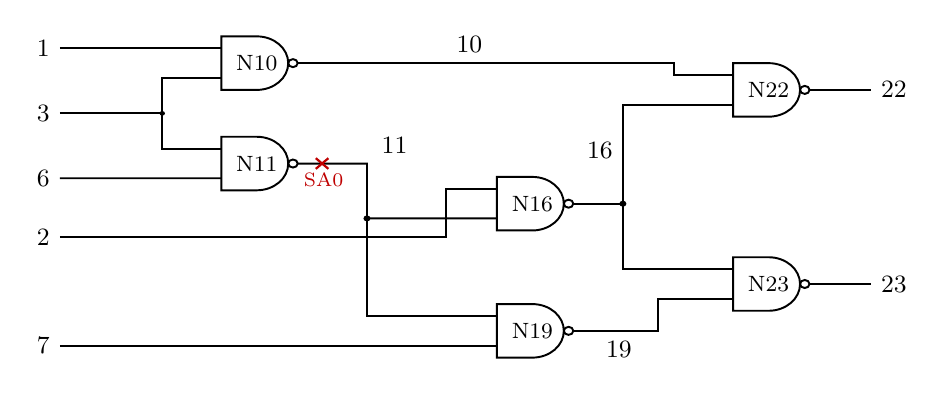
\begin{tikzpicture}[x=1cm,y=0.85cm,line width=0.7pt,
 every node/.style={font=\ifPOneVal\large\else\small\fi},
 nand/.pic={
 \draw (-0.45,-0.4)--(-0.45,0.4)--(0,0.4)
 arc[start angle=90,end angle=-90,radius=0.4]--cycle;
 \draw (0.46,0) circle[radius=0.06];
 \coordinate (-a) at (-0.45,0.22);
 \coordinate (-b) at (-0.45,-0.22);
 \coordinate (-out) at (0.52,0);}]
\ifPOneVal\tikzset{lp/.style={red!75!black,very thick},lc/.style={red!75!black}}%
\else\tikzset{lp/.style={},lc/.style={}}\fi
\pic (g10) at (2.5,4) {nand};
\pic (g11) at (2.5,2.5) {nand};
\pic (g16) at (6,1.9) {nand};
\pic (g19) at (6,0) {nand};
\pic (g22) at (9,3.6) {nand};
\pic (g23) at (9,0.7) {nand};
\foreach \id/\x/\y in {10/2.5/4,11/2.5/2.5,16/6/1.9,19/6/0,22/9/3.6,23/9/0.7}
 \node[font=\footnotesize] at (\x,\y) {N\id};
\node[left] at (0,4.22) {\POneLab{1}{$1=X$}};
\node[left] at (0,3.25) {\POneLab{3}{$3=0$}};
\node[left] at (0,2.28) {\POneLab{6}{$6=X$}};
\node[left] at (0,1.4) {\POneLab{2}{$2=1$}};
\node[left] at (0,-0.22) {\POneLab{7}{$7=X$}};
\draw (0,4.22)--(g10-a);
\draw (0,3.25)--(1.3,3.25);
\draw (1.3,3.25)|-(g10-b);
\draw (1.3,3.25)|-(g11-a);
\fill (1.3,3.25) circle[radius=0.035];
\draw (0,2.28)--(g11-b);
\draw (0,1.4)--(4.9,1.4)|-(g16-a);
\draw (0,-0.22)--(g19-b);
\draw (g10-out)--(7.8,4)|-(g22-a);
\node[above] at (5.2,4) {\POneLab{10}{$10=1$}};
\draw[lp] (g11-out)--(3.9,2.5)--(3.9,1.68)--(g16-b);
\draw (3.9,1.68)|-(g19-a);
\fill[lc] (3.9,1.68) circle[radius=0.045];
\node[above,lc] at (4.25,2.5) {\POneLab{11}{$11=D$}};
\node[below,font=\scriptsize,red!75!black] at (3.35,2.5) {SA0};
\draw[red!75!black,thick] (3.25,2.42)--(3.41,2.58) (3.25,2.58)--(3.41,2.42);
\draw[lp] (g16-out)--(7.15,1.9)|-(g22-b);
\draw (7.15,1.9)|-(g23-a);
\fill[lc] (7.15,1.9) circle[radius=0.045];
\node[left,lc] at (7.15,2.7) {\POneLab{16}{$16=D'$}};
\draw (g19-out)--(7.6,0)|-(g23-b);
\node[below] at (7.1,0) {\POneLab{19}{$19=X$}};
\draw[lp] (g22-out)--(10.3,3.6);
\node[right,lc] at (10.3,3.6) {\POneLab{22}{$22=D$}};
\draw (g23-out)--(10.3,0.7);
\node[right] at (10.3,0.7) {\POneLab{23}{$23=X$}};
\end{tikzpicture}}

\begin{frame}{Mạch ví dụ chung: c17 và lỗi 11/SA0}
\centering
\POneValfalse
\resizebox{0.86\textwidth}{!}{\POneCseventeen}
\par\medskip
\small 6 cổng NAND; 5 ngõ vào $1,2,3,6,7$; 2 ngõ ra $22,23$.
Lỗi cần tìm: \textcolor{red!75!black}{net 11 kẹt ở 0}.
\end{frame}

\begin{frame}{Kích hoạt và lan truyền lỗi 11/SA0}
\begin{columns}[c,onlytextwidth]
\column{0.57\textwidth}
\centering
\POneValtrue
\resizebox{\linewidth}{!}{\POneCseventeen}
\column{0.41\textwidth}
\footnotesize
\begin{enumerate}
\item \textbf{Kích hoạt:} đặt $3=0$ \(\Rightarrow\) $11=\overline{3\cdot6}$:
 tốt 1, lỗi 0, tức $11=D$.
\item \textbf{Lan truyền:} đặt $2=1$ \(\Rightarrow\)
 $16=\overline{2\cdot11}=D'$; đồng thời $10=\overline{1\cdot3}=1$.
\item $22=\overline{10\cdot16}=D$: \textbf{quan sát được lỗi} ở ngõ ra.
\end{enumerate}
\begin{block}{Mẫu theo thứ tự PI $(1,2,3,6,7)$}
$(X,1,0,X,X)$; điền $X=0$ được $01000$.
\end{block}
\end{columns}
\end{frame}

\begin{frame}{Lộ trình và tiêu chí kiểm chứng}
\begin{itemize}
\item D-algorithm và PODEM; cùng minh họa lỗi c17 11/SA0.
\item ATPG tuần tự: trạng thái, full scan và trải khung thời gian.
\item Cài đặt, trace, mô phỏng lỗi và coverage.
\item Coverage phải ghi rõ danh sách lỗi; hết giới hạn tìm kiếm là
\texttt{ABORTED}, không kết luận \texttt{UNTESTABLE}.
\end{itemize}
\begin{block}{Bài tập trong giáo trình (video 2--3 phút)}
Ví dụ Hình 4.5: $f=xy+\overline y z$, tìm mẫu cho $y/SA0$.
\end{block}
\end{frame}
